\documentclass[11pt]{article}

\usepackage[margin=1in]{geometry}
\usepackage{amsmath,amssymb,amsthm}
\usepackage{bm}
\usepackage{mathtools}
\usepackage{xcolor}
\usepackage{graphicx}
\usepackage{subcaption}
\usepackage{booktabs}
\graphicspath{{panels/}}
\usepackage{hyperref}
\hypersetup{colorlinks=true,linkcolor=blue,citecolor=blue,urlcolor=blue}
\emergencystretch=2.5em  % absorb residual overfull boxes from long \texttt names

\newcommand{\dt}{\Delta t}
\newcommand{\Nf}{N_f}
\newcommand{\Nt}{N_t}
\newcommand{\Ntl}{N_\ell}
\newcommand{\re}{\operatorname{Re}}
\newcommand{\im}{\operatorname{Im}}
\newcommand{\ip}[2]{\left\langle #1 \,\middle|\, #2 \right\rangle}
\newcommand{\cc}{c'}
\newcommand{\invC}{(\bm{C}^{-1})}
\newcommand{\Cmn}{\mathcal{C}}

\title{\bf The signal--heterodyne (sig--het) likelihood for galactic binaries\\
\large WDM--domain polyphase heterodyne with a real--projection bin--fold}
\author{LISA sprint 2026 --- GB chunked/signal--het work item}
\date{\today}

\begin{document}
\maketitle

\begin{abstract}
This note documents the mathematics of the \emph{signal--heterodyne} (sig--het)
galactic--binary (GB) likelihood implemented in
\texttt{gbsignalhetcomputations.py} / \texttt{gb\_signal\_het\_wdm\_v2.py} and the
backing C\texttt{++} kernel
\texttt{gb\_signal\_het\_get\_ll\_in\_kernel}. The method evaluates the
Wilson--Daubechies--Meyer (WDM) wavelet--domain log--likelihood of a near
monochromatic GB without ever forming the dense WDM template. It rests on three
ideas: (i) a \emph{heterodyne} factorization of the candidate template against a
fixed reference, (ii) a \emph{polyphase} per--layer minimal--length inverse FFT
that produces the candidate WDM coefficients only on a sparse time grid, and
(iii) a \emph{linearized bin--fold} that pre--contracts the data and reference
into per--bin coefficients so each likelihood call is a handful of cheap sums.
We also derive the \emph{real--WDM projection} that removes the spurious
$\sim\!10^{-3}$ accuracy floor present in the original complex/Hermitian
bin--fold.
\end{abstract}

\tableofcontents

\section{The WDM--domain likelihood}

LISA TDI data $d_c(t)$ in channels $c\in\{X,Y,Z\}$ (or $\{A,E,T\}$) are sampled
at cadence $\dt$ over $N=\Nf\Nt$ samples. The Gaussian log--likelihood for a
template $h_c(\bm\theta)$ is
\begin{equation}
\ln\mathcal{L}(\bm\theta)
   \;=\; \ip{d}{h} \;-\; \tfrac12\,\ip{h}{h} \;-\; \tfrac12\,\ip{d}{d},
\label{eq:logL}
\end{equation}
with a noise--weighted inner product. We work in the \emph{WDM wavelet domain}:
a real time series $x_c(t)$ is mapped to real coefficients $w^{x}_{cmn}$ on a
time--frequency lattice indexed by a frequency layer $m$ and a time pixel $n$.
The layer spacing is $\Delta f = 1/(2\Nf\dt)$ and the pixel spacing is
$\Delta\tau = \Nf\dt$. In this basis the inner product is diagonal in $(m,n)$
and reduces to a sensitivity--weighted sum,
\begin{equation}
\ip{a}{b}
  \;=\; \sum_{m,n}\ \sum_{c,\cc}\,
        w^{a}_{cmn}\,\invC_{c\cc mn}\,w^{b}_{\cc mn},
\label{eq:ip-real}
\end{equation}
where $\invC_{c\cc mn}$ is the inverse noise covariance (the inverse of the
per--pixel cross--channel sensitivity matrix; for diagonal $\{A,E,T\}$ it
collapses to a scalar $\invC_{cmn}$). All overall factors ($4\,\mathrm{d}c$,
quadrature weights) are folded into $\invC$ so that \eqref{eq:ip-real} is exact
against the lisatools \texttt{template\_likelihood}.

\paragraph{Why this is hard for a GB.} A galactic binary is nearly
monochromatic: its power sits in $\lesssim 5$ frequency layers around the
carrier $f_0$, but spread across \emph{all} $\Nt$ time pixels. A brute--force
likelihood forms the dense $w^h_{cmn}$ for every candidate $\bm\theta$ via a
length--$\Nt$ inverse FFT per layer --- the dominant cost in an MCMC. The
sig--het method removes that cost.

\section{The complex (quadrature) WDM transform}
\label{sec:wdm}

It is convenient to use the \emph{complex} (quadrature) WDM transform, whose
coefficients $\Cmn^{x}_{cmn}\in\mathbb{C}$ carry both the cosine-- and
sine--phase of the wavelet response. Writing $\hat x_c(k)=\sum_{l}x_c(l)\,
e^{-2\pi i k l/N}$ for the length--$N$ DFT of the (windowed) channel, the
coefficient at layer $m$, pixel $n$ is
\begin{equation}
\Cmn^{x}_{cmn}
  \;=\; \kappa\, s_{mn}\,\bar\Cmn_{mn}\,\sqrt{\dt}\;
        \underbrace{\frac{1}{\Nt}\sum_{j=-\Nt/2}^{\Nt/2-1}
        \tilde\Phi(j)\;\hat x_c\!\Big(m\tfrac{\Nt}{2}+j\Big)\,
        e^{\,2\pi i\,j\,n/\Nt}}_{\displaystyle \equiv\,G^{x}_{cmn}},
\label{eq:wdm-def}
\end{equation}
with the normalisation and phase factors
\begin{align}
\kappa &= \frac{2\sqrt{\pi}}{\Nf}, &
s_{mn} &= (-1)^{(m+1)n}, &
\bar\Cmn_{mn} &=
  \begin{cases} 1, & m+n \ \text{even},\\[2pt] -i, & m+n\ \text{odd}, \end{cases}
\label{eq:wdm-factors}
\end{align}
and $\tilde\Phi$ the Meyer analysis window
\begin{equation}
\tilde\Phi(\omega) = \frac{1}{\sqrt{\Delta\Omega}}\times
\begin{cases}
1, & |\omega|<A,\\[2pt]
\cos\!\Big[\tfrac{\pi}{2}\,I_{p,p}\!\big(\tfrac{|\omega|-A}{B}\big)\Big],
  & A\le|\omega|<A+B,\\[2pt]
0, & \text{otherwise,}
\end{cases}
\qquad
\begin{aligned}
\Delta\Omega&=\pi/\Nf,\\
A&=\Delta\Omega/4,\ B=\Delta\Omega-2A,
\end{aligned}
\label{eq:phitilde}
\end{equation}
evaluated at $\omega=2\pi j/N$, where $I_{p,p}$ is the regularised incomplete
beta function with $p=4$. The window has support $|j|<\Nt/2$ FD bins, so the
natural gather length is exactly $\Nt$. The layer centre maps to DFT bin
$m\,\Nt/2$ because the layer frequency $m\Delta f$ corresponds to bin
$m\Delta f\,(N\dt)=m\Nt/2$.

\paragraph{The bridge to the real likelihood.} The real WDM coefficient used in
\eqref{eq:ip-real} is exactly the real part of the complex one,
\begin{equation}
\boxed{\;w^{x}_{cmn} \;=\; \re\,\Cmn^{x}_{cmn}\;}
\label{eq:re-bridge}
\end{equation}
term for term. Equation~\eqref{eq:re-bridge} is the linchpin of
Section~\ref{sec:realproj}: the likelihood is a quadratic form in
$\re\,\Cmn$, \emph{not} in $|\Cmn|$.

\begin{figure}[htbp]
\centering
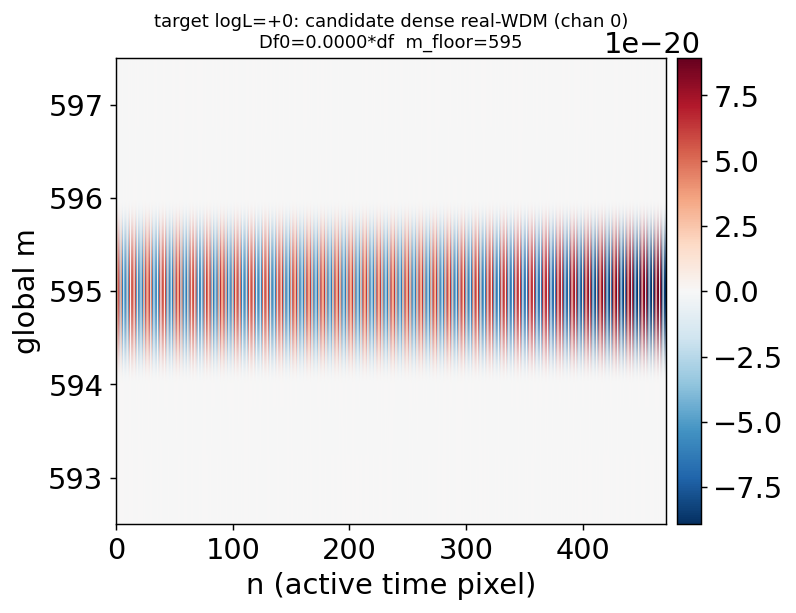
\includegraphics[width=0.62\textwidth]{panel_rank0_r0_c0_dense}
\caption{The (real) WDM coefficients $w_{cmn}=\re\,\Cmn_{cmn}$ of a galactic
binary on the active frequency band $m_0\pm M$ ($M=2$), for the highest--frequency
mojito source ($f_0=20.38$\,mHz, channel $X$). Power sits in the carrier layer
$m_0$ and its two neighbours and runs across every time pixel $n$ --- this is the
object the dense likelihood forms per candidate, and the one the sig--het method
avoids building.}
\label{fig:dense}
\end{figure}

\section{Heterodyne factorization}
\label{sec:het}

Fix a \emph{reference} parameter vector $\bm\theta_0$ (in practice the catalogue
source, or the current MCMC mode) and precompute its dense complex WDM
coefficients once,
\begin{equation}
c^0_{cmn} \;\equiv\; \Cmn^{h(\bm\theta_0)}_{cmn}.
\end{equation}
For a candidate $\bm\theta$ with complex WDM $c^1_{cmn}\equiv
\Cmn^{h(\bm\theta)}_{cmn}$, define the per--pixel \emph{heterodyne ratio}
\begin{equation}
r_{cmn} \;\equiv\; \frac{c^1_{cmn}}{c^0_{cmn}}
\qquad(\text{where } |c^0_{cmn}| \ \text{is above a small floor}).
\label{eq:ratio}
\end{equation}
For a candidate close to the reference, $r_{cmn}$ is a slowly varying function of
the time pixel $n$ within each layer: the rapid pixel--to--pixel oscillation of
the GB carrier is shared by $c^1$ and $c^0$ and cancels in the ratio, leaving a
smooth low--order phase/amplitude drift (a near--linear wind in $n$ set by the
carrier mismatch $\Delta f_0$). This is the property the bin--fold exploits.
The candidate template is recovered as $c^1_{cmn}=r_{cmn}\,c^0_{cmn}$, i.e.\
$h_{cmn}=r_{cmn}\,c^0_{cmn}$.

\begin{figure}[htbp]
\centering
\begin{subfigure}[t]{0.49\textwidth}
  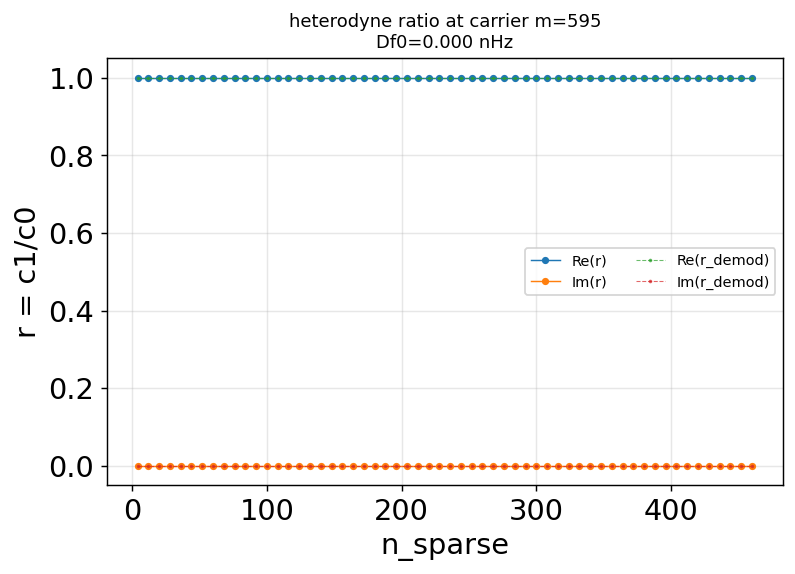
\includegraphics[width=\textwidth]{panel_rank0_r0_c2_ratio}
  \caption{$\ln\mathcal L=0$ (candidate $=$ reference): $r\equiv1$.}
\end{subfigure}\hfill
\begin{subfigure}[t]{0.49\textwidth}
  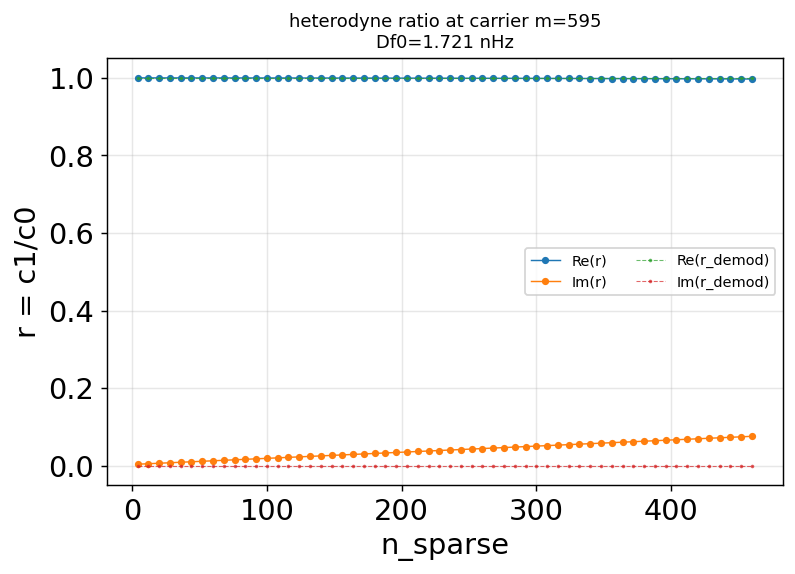
\includegraphics[width=\textwidth]{panel_rank0_r1_c2_ratio}
  \caption{$\ln\mathcal L\approx-5$: gentle wind.}
\end{subfigure}

\vspace{0.6em}
\begin{subfigure}[t]{0.49\textwidth}
  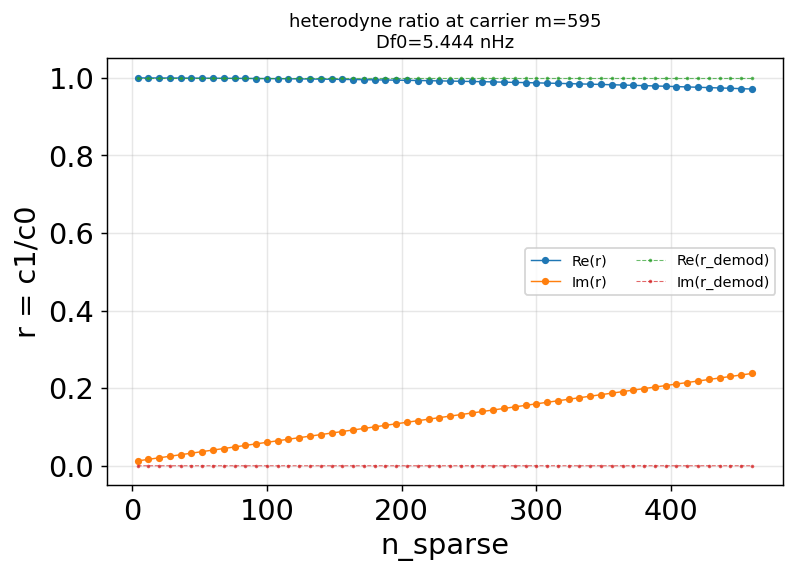
\includegraphics[width=\textwidth]{panel_rank0_r2_c2_ratio}
  \caption{$\ln\mathcal L\approx-50$.}
\end{subfigure}\hfill
\begin{subfigure}[t]{0.49\textwidth}
  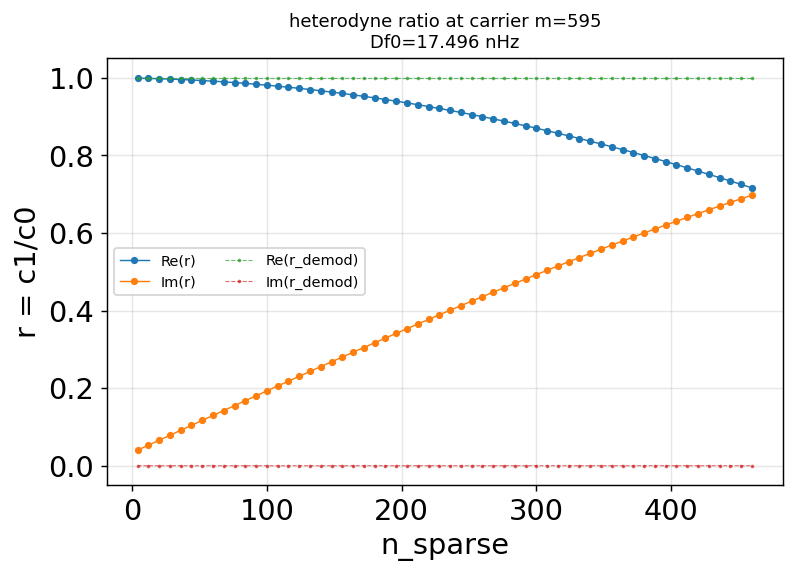
\includegraphics[width=\textwidth]{panel_rank0_r3_c2_ratio}
  \caption{$\ln\mathcal L\approx-500$: full half--turn.}
\end{subfigure}
\caption{The heterodyne ratio $r_{cm}(n)=c^1/c^0$ at the carrier layer $m=m_0$, as
the candidate $f_0$ is walked away from the reference (the four sig--het rows of
the explainer, mojito rank~0). At the peak $r\equiv1$; off the reference it
becomes a smooth, near--linear \emph{wind} in $n$ set by the carrier mismatch
$\Delta f_0$ (blue/orange $=\re/\im r$). The de--rotated $r_{\rm demod}=r\,
e^{-2\pi i\,\Delta f_0\,t_n}$ (green/red) removes that ramp and stays flat,
confirming the slow variation the linearized bin--fold \eqref{eq:lin}
exploits.}
\label{fig:ratio}
\end{figure}

\section{Sparse polyphase evaluation of the candidate}
\label{sec:polyphase}

We only ever need $c^1$ on the active frequency layers $m\in\mathcal{M}=
\{m_0-M,\dots,m_0+M\}$ (with $m_0=\lfloor f_0/\Delta f\rfloor$ and half--width
$M$, default $M=2$) and on a \emph{sparse} time grid
\begin{equation}
n_b = \nu + b\,\sigma,\qquad b=0,\dots,N_b-1,\qquad
\sigma=\Nt/\Ntl,
\label{eq:sparsegrid}
\end{equation}
i.e.\ every $\sigma$--th pixel, with $\sigma$ the \emph{stride} and $\Ntl$ the
per--layer FFT length. The inner factor $G^{x}_{cmn}$ in \eqref{eq:wdm-def} is a
length--$\Nt$ inverse DFT; evaluating it only on the strided grid lets us
replace it by a length--$\Ntl$ inverse DFT.

\paragraph{Polyphase identity.} Write the windowed, pre--phased FD samples as
\begin{equation}
W_j \;=\; \tilde\Phi(j)\,\hat x_c\!\Big(m\tfrac{\Nt}{2}+j\Big),
\qquad j=0,\dots,\Nt-1
\end{equation}
(absorbing the centring shift into the index). We want
$G(n)=\tfrac1{\Nt}\sum_{j=0}^{\Nt-1}W_j\,e^{2\pi i j n/\Nt}$ at
$n=\nu+b\,\sigma$. Split $e^{2\pi i j n/\Nt}=e^{2\pi i j\nu/\Nt}\,
e^{2\pi i j b/\Ntl}$ (using $\sigma/\Nt=1/\Ntl$) and absorb the first exponential
into a \emph{pre--phase}, $\tilde W_j = W_j\,e^{2\pi i j\nu/\Nt}$. Decomposing
$j=q\Ntl+\rho$ with $q=0,\dots,\sigma-1$ and $\rho=0,\dots,\Ntl-1$, and using
$e^{2\pi i q\Ntl b/\Ntl}=1$,
\begin{equation}
G(\nu+b\sigma)
   = \frac{1}{\Nt}\sum_{\rho=0}^{\Ntl-1}
     \underbrace{\Big(\sum_{q=0}^{\sigma-1}\tilde W_{q\Ntl+\rho}\Big)}_{\displaystyle Y_\rho}
     e^{2\pi i\rho b/\Ntl}
   \;=\; \frac{1}{\sigma}\,\mathrm{IDFT}_{\Ntl}\!\big[Y\big]_b .
\label{eq:polyphase}
\end{equation}
So: \emph{fold} the length--$\Nt$ pre--phased window into length $\Ntl$ by summing
the $\sigma$ polyphase branches, run \emph{one} length--$\Ntl$ inverse FFT, and
scale by $1/\sigma$. This is mathematically exact for any $\sigma$ dividing
$\Nt$ --- the only approximation in the whole method is the bin--fold
linearization of Section~\ref{sec:binfold}, never the polyphase step. The
per--layer cost drops from $\mathcal{O}(\Nt\log\Nt)$ to
$\mathcal{O}(\Ntl\log\Ntl)$.

Restoring the WDM dressing of \eqref{eq:wdm-def}, the sparse candidate
coefficient is
\begin{equation}
c^1_{c m n_b}
  = \sqrt{\dt}\;\kappa\,s_{m n_b}\,\bar\Cmn_{m n_b}\,
    \frac{1}{\sigma}\,\mathrm{IDFT}_{\Ntl}\!\big[Y^{(c,m)}\big]_b .
\end{equation}
The Hermitian wrap $\hat x_c(-k)=\hat x_c^{*}(k)$ (real time series) supplies the
negative--frequency window bins; the reference $c^0$ is computed once by the
ordinary dense transform.

\begin{figure}[htbp]
\centering
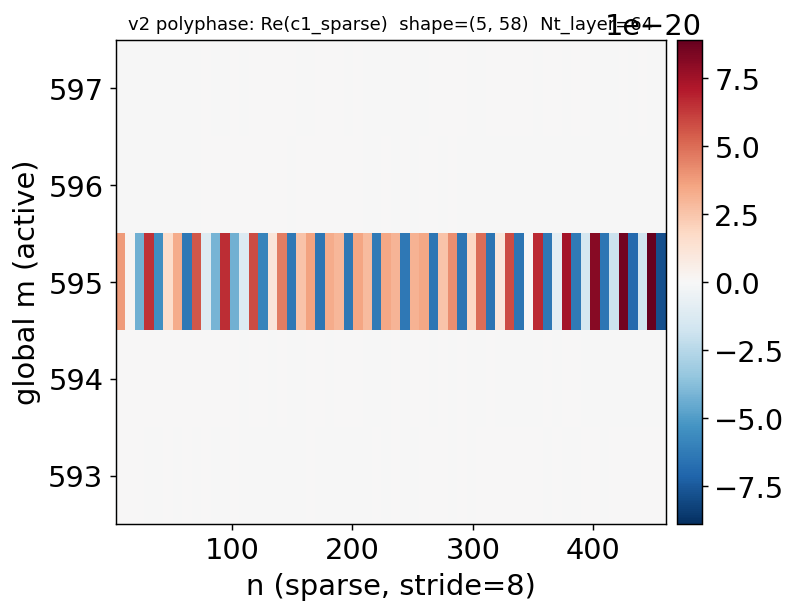
\includegraphics[width=0.62\textwidth]{panel_rank0_r0_c1_sparse}
\caption{The sparse complex--WDM coefficients $\re\,c^1_{cmn_b}$ produced by the
polyphase step \eqref{eq:polyphase} for the same source, on the active
layers ($5$ rows) and the strided time grid ($\sigma=8$, so $N_b=58$ columns).
A single length--$\Ntl$ inverse FFT per layer replaces the length--$\Nt$ dense
transform of Fig.~\ref{fig:dense}; the result is exact (per--pixel relative
difference $<10^{-12}$) at the sparse pixels.}
\label{fig:sparse}
\end{figure}

\paragraph{Choosing $\Ntl$.} Polyphase is exact at any valid $\Ntl$, but the
stride $\sigma=\Nt/\Ntl$ sets the spacing of the sparse grid on which $r$ is
sampled. $\Ntl$ is auto--calibrated at construction by increasing
$\Ntl\in\{16,32,64,\dots\}$ until the sparse output matches the dense lisatools
reference to a per--pixel relative difference $<10^{-12}$, and so that $r$ is
well represented by a line over $\sigma$ pixels (typically $\sigma\lesssim16$).

\section{Linearized bin--fold of the inner products}
\label{sec:binfold}

The inner products \eqref{eq:ip-real} are sums over \emph{all} pixels $n$, but we
have $r$ only at the sparse centres $n_b$. Within bin $b$ (the pixels $n$ closest
to $n_b$) we linearise the smooth ratio,
\begin{equation}
r_{cmn} \;\approx\; r_{cm}(n_b) \;+\; \dot r_{cm}(n_b)\,(n-n_b),
\qquad
\dot r_{cm}(n_b) = \frac{r_{cm}(n_{b+1})-r_{cm}(n_{b-1})}{2\,\overline{\Delta n}},
\label{eq:lin}
\end{equation}
with $\overline{\Delta n}$ the mean bin width (one--sided differences at the
ends). The template enters the inner products only through $h_{cmn}=r_{cmn}\,
c^0_{cmn}$, so substituting \eqref{eq:lin} lets us pre--contract everything that
does \emph{not} depend on $\bm\theta$ --- the data $d$, the reference $c^0$, and
$\invC$ --- into per--bin coefficients. This is the key move: the expensive
all--pixel sums are done \emph{once}, at construction; each likelihood call only
sums over the $N_b$ sparse bins.

We give the contraction directly in its real--projection form
(Section~\ref{sec:realproj} explains why this, and not the naive complex form, is
correct).

\section{Real--WDM projection and the inner products}
\label{sec:realproj}

\subsection{The complex--vs--real subtlety}

By \eqref{eq:re-bridge} the likelihood is a quadratic form in $\re\,\Cmn$.
A natural but \emph{wrong} shortcut is to evaluate the Hermitian complex form
\begin{equation}
\tfrac12\re\sum_{c\cc mn} \Cmn^{a\,*}_{cmn}\,\invC_{c\cc mn}\,\Cmn^{b}_{\cc mn}
  = \tfrac12\sum_{c\cc mn}\invC_{c\cc mn}
    \big(\re\Cmn^a\,\re\Cmn^b + \im\Cmn^a\,\im\Cmn^b\big),
\label{eq:hermitian}
\end{equation}
which carries a spurious $\im\!\cdot\!\im$ term relative to the true real form
$\sum \re\Cmn^a\,\invC\,\re\Cmn^b$. The two agree only when
$\sum\im^2\approx\sum\re^2$ by phase averaging, which holds for the broadband
$\ip{d}{d}$ but \emph{not} pixel--by--pixel in the bin--fold. The residual
\begin{equation}
\tfrac12\sum\invC\,\big(\im\Cmn^a\,\im\Cmn^b-\re\Cmn^a\,\re\Cmn^b\big)
\end{equation}
is exactly the $\sim\!6.5\times10^{-3}$ effective--mismatch floor observed in the
original sig--het. The fix is to project each coefficient to its real part
\emph{before} contracting.

\subsection{Real projection of $\langle d|h\rangle$}

Write $u_{cmn}=\re\,c^0_{cmn}$, $v_{cmn}=\im\,c^0_{cmn}$, so that with
$h=r\,c^0$,
\begin{equation}
\re\,h_{cmn} \;=\; u_{cmn}\,\re\,r_{cmn} \;-\; v_{cmn}\,\im\,r_{cmn}.
\label{eq:Reh}
\end{equation}
The (real) data--template term is, using \eqref{eq:ip-real},
\begin{equation}
\ip{d}{h}
  = \sum_{mn}\sum_{c\cc}\re d_{cmn}\,\invC_{c\cc mn}\,\re h_{\cc mn}
  = \sum_{mn}\sum_{\cc}\, D^{\re}_{\cc mn}\,
    \big(u_{\cc mn}\re r_{\cc mn}-v_{\cc mn}\im r_{\cc mn}\big),
\end{equation}
with the data pre--contraction $D^{\re}_{\cc mn}=\sum_{c}\re d_{cmn}\,
\invC_{c\cc mn}$ (a scalar $\re d_{cmn}\invC_{cmn}$ in the diagonal case).
Inserting the linearization \eqref{eq:lin} and bin--folding gives, per channel
$\cc$, layer $m$, bin $b$, the two real moment pairs
\begin{equation}
A_0^{\re}=\!\!\sum_{n\in b}\! D^{\re}u,\quad
A_0^{\im}=\!\!\sum_{n\in b}\! D^{\re}v,\quad
A_1^{\re}=\!\!\sum_{n\in b}\! D^{\re}u\,(n-n_b),\quad
A_1^{\im}=\!\!\sum_{n\in b}\! D^{\re}v\,(n-n_b).
\end{equation}
The crucial repacking is to store these as \emph{single complex} coefficients
\begin{equation}
\boxed{\;A_0 = 2\big(A_0^{\re}+iA_0^{\im}\big),\qquad
        A_1 = 2\big(A_1^{\re}+iA_1^{\im}\big),\;}
\label{eq:A0repack}
\end{equation}
because then the \emph{existing} complex kernel contraction reproduces the real
value at no extra storage:
\begin{equation}
\tfrac12\re\!\sum_{\cc mb}\!\big(A_0\,r + A_1\,\dot r\big)
 = \sum_{\cc mb}\!\big(A_0^{\re}\re r - A_0^{\im}\im r
   + A_1^{\re}\re\dot r - A_1^{\im}\im\dot r\big)
 = \ip{d}{h}.
\label{eq:dh-final}
\end{equation}
The middle identity uses $\tfrac12\re[2(A_0^{\re}+iA_0^{\im})(\re r+i\im r)]
=A_0^{\re}\re r-A_0^{\im}\im r$.

\subsection{Real projection of $\langle h|h\rangle$}

The template norm is genuinely quadratic in $r$, so a single complex coefficient
cannot absorb it; two blocks are needed. Using \eqref{eq:Reh},
\begin{equation}
\ip{h}{h}=\sum_{mn}\sum_{c\cc}\invC_{c\cc mn}\,\re h_{cmn}\,\re h_{\cc mn},
\end{equation}
and the algebraic identity (with $h=r\,c^0$, valid for symmetric $\invC$)
\begin{equation}
2\,\re h_{c}\,h_{\cc}
 = \underbrace{c^{0\,*}_{c}\,\invC\,c^0_{\cc}}_{\text{conj}}\,r_c^{*}r_{\cc}
   + \underbrace{c^0_{c}\,\invC\,c^0_{\cc}}_{\text{non--conj}}\,r_c r_{\cc}
\end{equation}
(after multiplying by $\invC$ and summing) motivates the \emph{two} bin--folded
blocks
\begin{align}
B_0 &= \sum_{n\in b} c^{0\,*}_{c}\,\invC_{c\cc}\,c^0_{\cc}, &
B_1 &= \sum_{n\in b} c^{0\,*}_{c}\,\invC_{c\cc}\,c^0_{\cc}\,(n-n_b), &&\text{(conj)}\\
B_0^{\mathrm{nc}} &= \sum_{n\in b} c^0_{c}\,\invC_{c\cc}\,c^0_{\cc}, &
B_1^{\mathrm{nc}} &= \sum_{n\in b} c^0_{c}\,\invC_{c\cc}\,c^0_{\cc}\,(n-n_b),
   &&\text{(non--conj)}
\end{align}
where for diagonal $\{A,E,T\}$ the channel pair $(c,\cc)$ collapses to one index.
The kernel then forms
\begin{equation}
\boxed{\;
\ip{h}{h}=\tfrac12\re\!\sum_{c\cc mb}\Big[
   B_0\,r_c^{*}r_{\cc} + B_0^{\mathrm{nc}}\,r_c r_{\cc}
 + B_1\big(r_c^{*}\dot r_{\cc}+\dot r_c^{*}r_{\cc}\big)
 + B_1^{\mathrm{nc}}\big(r_c\dot r_{\cc}+\dot r_c r_{\cc}\big)\Big].\;}
\label{eq:hh-final}
\end{equation}
To see that \eqref{eq:hh-final} is the real norm, note (suppressing $m,b$ and
writing $r_c=a_c+ib_c$, $c^0_c=u_c+iv_c$, so $h_c=c^0_c r_c$):
\begin{equation}
B_0\,r_c^{*}r_{\cc}+B_0^{\mathrm{nc}}\,r_c r_{\cc}
 = \invC_{c\cc}\big(h_c^{*}h_{\cc}+h_c h_{\cc}\big)
 = \invC_{c\cc}\,h_{\cc}\,(2\re h_c),
\end{equation}
and taking $\tfrac12\re$ leaves $\sum\invC_{c\cc}\re h_c\,\re h_{\cc}=\ip{h}{h}$
(the $B_1$ blocks carry the same identity for the linearization slope). The
non--conjugated blocks are the only new storage versus the original Hermitian
form. Dropping the $\dot r^2$ (second--order, $(n-n_b)^2$) term keeps $\ip{h}{h}$
to the standard linear--in--$r$ budget off the reference --- exact at
$\bm\theta=\bm\theta_0$ and tracking the dense WDM likelihood to
$\lesssim10^{-2}$ in $\ln\mathcal L$ even hundreds of units away from the peak.
A flag \texttt{project\_real} selects this path; with it disabled the kernel
reproduces the old complex form \eqref{eq:hermitian} bit for bit.

\section{Assembled likelihood and algorithm}

Collecting \eqref{eq:dh-final} and \eqref{eq:hh-final}, the log--likelihood is
\begin{equation}
\ln\mathcal{L}(\bm\theta)
 = \tfrac12\re\!\sum_{\cc mb}\!\big(A_0 r+A_1\dot r\big)
 \;-\;\tfrac12\cdot\tfrac12\re\!\sum_{c\cc mb}\!\big[\cdots\big]_{\eqref{eq:hh-final}}
 \;-\;\tfrac12\,\ip{d}{d},
\label{eq:logL-final}
\end{equation}
with $\ip{d}{d}$ a fixed scalar from the (real) lisatools data inner product. The
two heterodyne terms are returned by the kernel as $\langle d|h\rangle$ and
$\langle h|h\rangle$; the frontend \texttt{GBSignalHetComputations.get\_ll} adds
$-\tfrac12\ip{d}{d}$ and returns $\ln\mathcal L$ directly.

\paragraph{Per likelihood call (the only $\bm\theta$--dependent work).}
\begin{enumerate}\itemsep2pt
\item Synthesize the candidate FD signal $\hat h_c(\bm\theta)$ (fast FD--direct GB
generator, or TD synth $+$ \texttt{rfft}).
\item For each active layer $m\in\mathcal{M}$: gather the $\Nt$ windowed FD bins,
apply the pre--phase, polyphase--fold to length $\Ntl$, one inverse FFT, dress
with $\kappa s_{mn}\bar\Cmn_{mn}\sqrt{\dt}$ --- giving $c^1_{cmn_b}$
[Eq.~\eqref{eq:polyphase}].
\item Form $r=c^1/c^0$ and $\dot r$ at the sparse centres
[Eqs.~\eqref{eq:ratio},\eqref{eq:lin}].
\item Contract against the precomputed $A_0,A_1,B_0,B_1,B_0^{\mathrm{nc}},
B_1^{\mathrm{nc}}$ to get $\langle d|h\rangle,\langle h|h\rangle$
[Eqs.~\eqref{eq:dh-final},\eqref{eq:hh-final}], then \eqref{eq:logL-final}.
\end{enumerate}

\paragraph{Once, at construction (independent of $\bm\theta$).} Build the data
WDM $d$ and reference $c^0=\Cmn^{h(\bm\theta_0)}$ on the active band; compute
$\ip{d}{d}$; bin--fold $D^{\re},u,v,\invC$ into
$A_0,A_1,B_0,B_1,B_0^{\mathrm{nc}},B_1^{\mathrm{nc}}$.

\section{Validation summary}

\begin{itemize}\itemsep2pt
\item \textbf{Polyphase} reproduces the dense lisatools complex WDM to
$<10^{-12}$ per pixel at any calibrated $\Ntl$ (it is algebraically exact).
\item \textbf{Real projection} lowers the effective mismatch floor from
$6.5\times10^{-3}$ (Hermitian) to $\sim\!2\times10^{-11}$ (kernel \texttt{project\_real=1} vs.\ \texttt{=0}).
\item \textbf{End--to--end vs.\ mojito data} (top three high--$f$ GBs,
$\Nt=512$; Table~\ref{tab:mojito}): the sig--het $\ln\mathcal L$ tracks the dense
lisatools $\ln\mathcal L$ to $\mathcal{O}(10^{-9})$ at the injection and
$\lesssim5\times10^{-2}$ out at $\ln\mathcal L=-500$, matching the
chunked--heterodyne path. Narrowband mismatches at the peak:
$\mathrm{mm5}\sim3\times10^{-11}$.
\end{itemize}

\begin{table}[htbp]
\centering
\caption{Absolute deviation $\big|\ln\mathcal L_{\rm sighet}-\ln\mathcal
L_{\rm base}\big|$ of the signal--het likelihood from the dense lisatools
likelihood, for the three highest--frequency mojito galactic binaries, with the
candidate $f_0$ walked to four target $\ln\mathcal L$ values
(Fig.~\ref{fig:ratio} shows the ratios for rank~0). Last column: narrowband
$\mathrm{mm5}$ at the peak. All likelihoods are taken from the installed
\texttt{get\_ll}/\texttt{template\_likelihood} methods.}
\label{tab:mojito}
\begin{tabular}{lccccc}
\toprule
& \multicolumn{4}{c}{$\big|\ln\mathcal L_{\rm sighet}-\ln\mathcal L_{\rm base}\big|$ at target $\ln\mathcal L=$} & \\
\cmidrule(lr){2-5}
Source (rank, $f_0$, SNR) & $0$ & $-5$ & $-50$ & $-500$ & $\mathrm{mm5}_{\rm peak}$ \\
\midrule
0\quad ($20.38$\,mHz, $57.6$) & $2.5\times10^{-8}$ & $2.9\times10^{-4}$ & $2.9\times10^{-3}$ & $2.3\times10^{-2}$ & $3.3\times10^{-11}$ \\
1\quad ($19.67$\,mHz, $23.8$) & $1.6\times10^{-9}$ & $4.8\times10^{-4}$ & $3.9\times10^{-3}$ & $8.2\times10^{-3}$ & $3.9\times10^{-11}$ \\
2\quad ($16.72$\,mHz, $61.1$) & $5.2\times10^{-9}$ & $5.9\times10^{-4}$ & $5.8\times10^{-3}$ & $5.3\times10^{-2}$ & $2.4\times10^{-11}$ \\
\bottomrule
\end{tabular}
\end{table}

\paragraph{Edge handling.} Both the sig--het and chunked paths use a WDM
time--edge cut $\ge$ the Tukey taper width $\lceil\alpha\Nt/2\rceil$ layers, so
their active time region matches the dense reference exactly; a mismatched cut
biases the absolute $\ln\mathcal L$ by a fixed fraction (different time
coverage), not the per--pixel floor that the real projection removed.

\end{document}
